\documentclass[10pt]{beamer}


% Matemáticas y Física
\usepackage{amsmath, amssymb}
\usepackage{mathtools}
\usepackage{bm}
\usepackage{physics}
\usepackage{cancel}
\usepackage{bbold}
\usepackage{mathpazo}
\usepackage{csquotes}

% Paquete para cajas personalizadas
\usepackage{tcolorbox}
\usepackage{xcolor}
\definecolor{VerdeEstimulo}{HTML}{27B13B}
\tcbuselibrary{skins}

% Definición del estilo de la caja para ecuaciones
\newtcolorbox{eqbox}{
    enhanced,
    colback=structure!5!white,        % Color de fondo (un gris/beige muy suave)
    colframe=structure, % Color de la barra vertical (tono verde/turquesa)
    arc=3mm,                % Radio de redondeo de las esquinas
    sharp corners=west,     % Esquinas izquierdas en ángulo recto (para la barra)
    boxrule=0pt,            % Elimina los bordes superior, inferior y derecho
    leftrule=3.5pt,         % Grosor de la barra lateral izquierda
    left=12pt,              % Margen interno entre la barra y el texto
    top=8pt,                % Margen interno superior
    bottom=8pt,             % Margen interno inferior
    width=\linewidth        % La caja ocupa todo el ancho de la columna
}

% Esto es obligatorio para que el estilo APA funcione bien
\usepackage[backend=biber, maxcitenames=2]{biblatex}
\addbibresource{bibliografia.bib}

% Gráficos y Tablas
\usepackage{soul}

% Preámbulo
\usetheme{Frankfurt} % tema de presentación
\usecolortheme{rose}
\usefonttheme{serif}
\useinnertheme{circles}
\setbeamertemplate{footline}[frame number]

% Datos de la presentación
\title{La Emergencia de Criticidad en Redes Neuronales Mediante el Aprendizaje}
\author{Olmo Viviens Blázquez}
\date{22 de julio de 2026}

\begin{document}

% Diapositiva de título
\begin{frame}
    \titlepage
\end{frame}

\begin{frame}
    \tableofcontents
\end{frame}

\section{Introducción}
\begin{frame}{Cerebro crítico e IA}
    Los nuevos métodos de toma de datos han mostrado que es probable que el cerebro trabaje en un régimen cercano a la {\color{blue}criticidad} \cite{beggs2003}, donde se ha mostrado que ciertos modelos de {\color{blue}IA} obtienen una {\color{blue}capacidad de análisis} óptima \cite{bertschinger2004}.
    \begin{columns}[c]
        \hfill
        \begin{column}{0.45\textwidth}
            Las claves para entender este fenómeno son:
            \begin{itemize}
                \item Criticidad Autoorganizada (SOC)
                \item Criticidad dinámica 
                \item Modelos de aprendizaje
            \end{itemize}
        \end{column}
        \hfill
        \begin{column}{0.45\textwidth}
            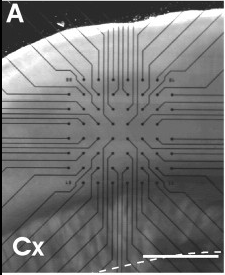
\includegraphics[width=.8\textwidth]{Figures/sensores.png}
        \end{column}
    \end{columns}

\end{frame}

\section{Fundamento teórico}

\begin{frame}{Criticidad Autoorganizada}
    \centering
    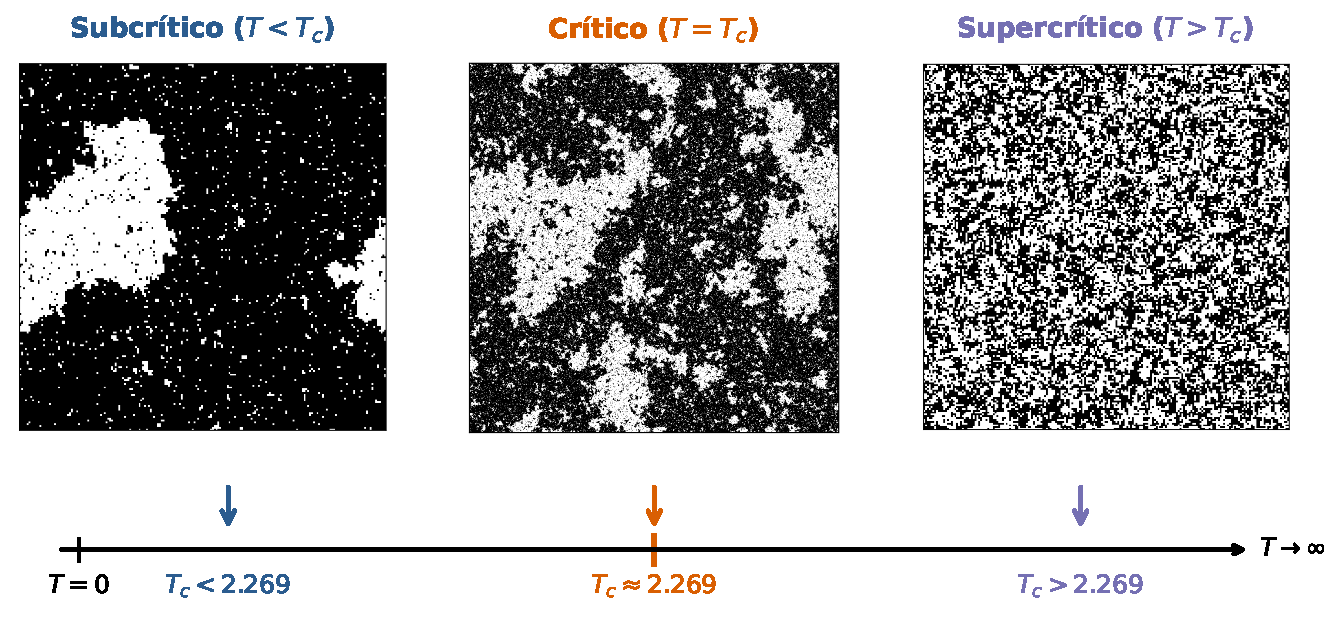
\includegraphics[width=\textwidth]{Figures/Ising_Temperaturas_Panel.pdf}
    
    Los sistemas con {\color{blue}criticidad autoorganizada} son capaces de posicionarse en el punto crítico de forma automática variando el {\color{blue}parámetro de control} en función del {\color{blue}parámetro de orden}. 
\end{frame}

\begin{frame}{Criticidad autoorganizada}
    Los sistemas con {\color{blue}criticidad autoorganizada} son inherentemente de {\color{blue}no equilibrio} y {\color{blue}dinámicos}, como

    \begin{itemize}
        \item Terremotos
        \item Incendios forestales
        \item Avalanchas
    \end{itemize}

    Dichos sistemas generan eventos {\color{blue}sin escala característica}, en los que se dan sucesos tanto mínimos como extremos. Vienen dados por distribuciones de {\color{blue}leyes de potencias}

    \begin{equation}
        P(S) = S^{-\tau}
    \end{equation}
\end{frame}

\begin{frame}{Criticidad Dinámica}
    La {\color{blue}criticidad dinámica} es una región de estabilidad de un sistema en la que la actividad de este no diverge, pero tampoco se estanca, sino que fluctua al {\color{blue}borde de la inestabilidad}. 
    
    \begin{columns}[b]
        \hfill
        \begin{column}{0.38\textwidth}
            El grado de estabilidad de un sistema viene dado por la parte real de los autovalores del jacobiano, siendo {\color{blue}inestable} cuando {\color{blue}\(\text{Re}(\lambda) > 0\)} y {\color{blue}estables} cuando {\color{blue}\(\text{Re}(\lambda) < 0\)}. La {\color{blue}criticidad dinámica} se da cuando {\color{blue}\(\text{Re}(\lambda) \approx 0\)}.
        \end{column}
        \begin{column}{0.6\textwidth}
                \centering
        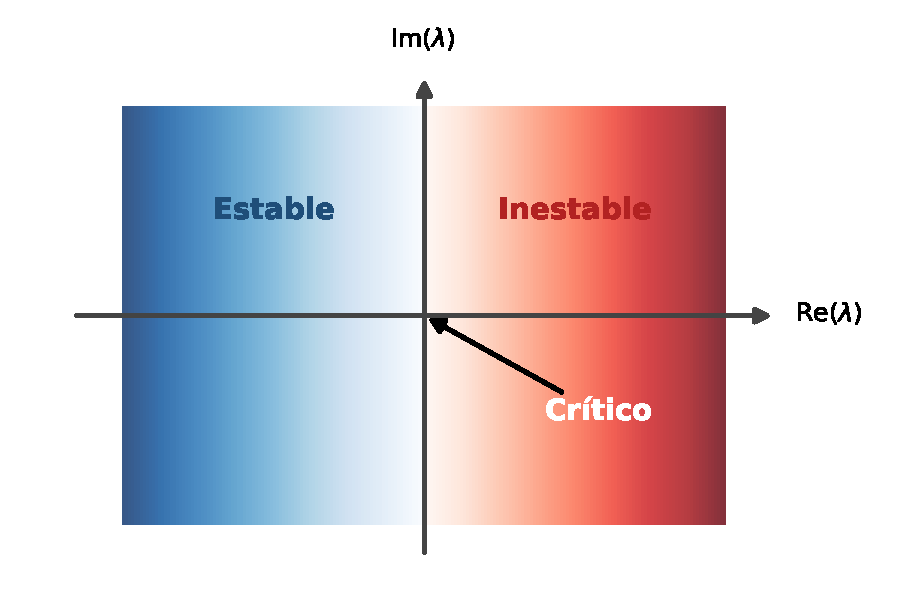
\includegraphics[width=\textwidth]{Figures/diagrama estabilidad anotado.pdf}
        \end{column}
    \end{columns}
    

\end{frame}

\begin{frame}{Aprendizaje Antihebbiano}
    Se va a simular una {\color{blue}red de \(N\) neuronas} interconectadas entre sí, donde la actividad de cada neurona afecta a la actividad del resto dependiendo de la conexón entre ellas.

    \begin{columns}
        \hfill
        \begin{column}{0.38\textwidth}
            \(\mathbf{x}\) representa el vector de {\color{blue}actividades} de cada una de las neuronas
            \begin{equation}
                \dot{\mathbf{x}} = W\mathbf{x}
            \end{equation}
            \(W\) representa las {\color{blue}conexiones} entre las neuronas\(\rightarrow\) \(W_{ij}\): conexión entre \(x_i\) y \(x_j\)
            \begin{equation}
                \dot{W} = \alpha (\mathbb{1} - \mathbf{xx}^T)
            \end{equation}
        \end{column}
        \begin{column}{0.6\textwidth}
            \centering 
            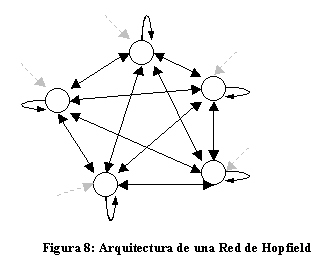
\includegraphics[width=\textwidth]{Figures/red.png}
        \end{column}
    \end{columns}
\end{frame}

\begin{frame}{Aprendizaje Antihebbiano}
    \begin{columns}[t]
        \begin{column}{0.48\textwidth}
            \textbf{\Large Evolución Actividad}
            La {\color{blue}actividad} de cada neurona depende de las otras mediante las conexiones entre ellas.
            \begin{eqbox}
                    \(\dot{\mathbf{x}} = W\mathbf{x}\)
            \end{eqbox}
        \end{column}
        \begin{column}{0.48\textwidth}
            \textbf{\Large Evolución Conexiones}
            Las {\color{blue}conexiones} entre dos neuronas disminuyen al aumentar la actividad de ambas.
            \begin{eqbox}
                \(\dot{W} = \alpha (\mathbb{1} - \mathbf{xx}^T)\)
            \end{eqbox}
        \end{column}
    \end{columns}

    \vfill

    Al aumentar la actividad, \(\mathbf{x}\), se genera un ciclo de retroalimentación negativa que frena las inestabilidades devolviendo las conexiones, \(W\), y la actividad, \(\mathbf{x}\), a 0, mientras que el término de la identidad evita la desaparición de las conexiones, \(W\).
\end{frame}

\section{Resultados}

\begin{frame}{Concentración de autovalores}
    \centering
    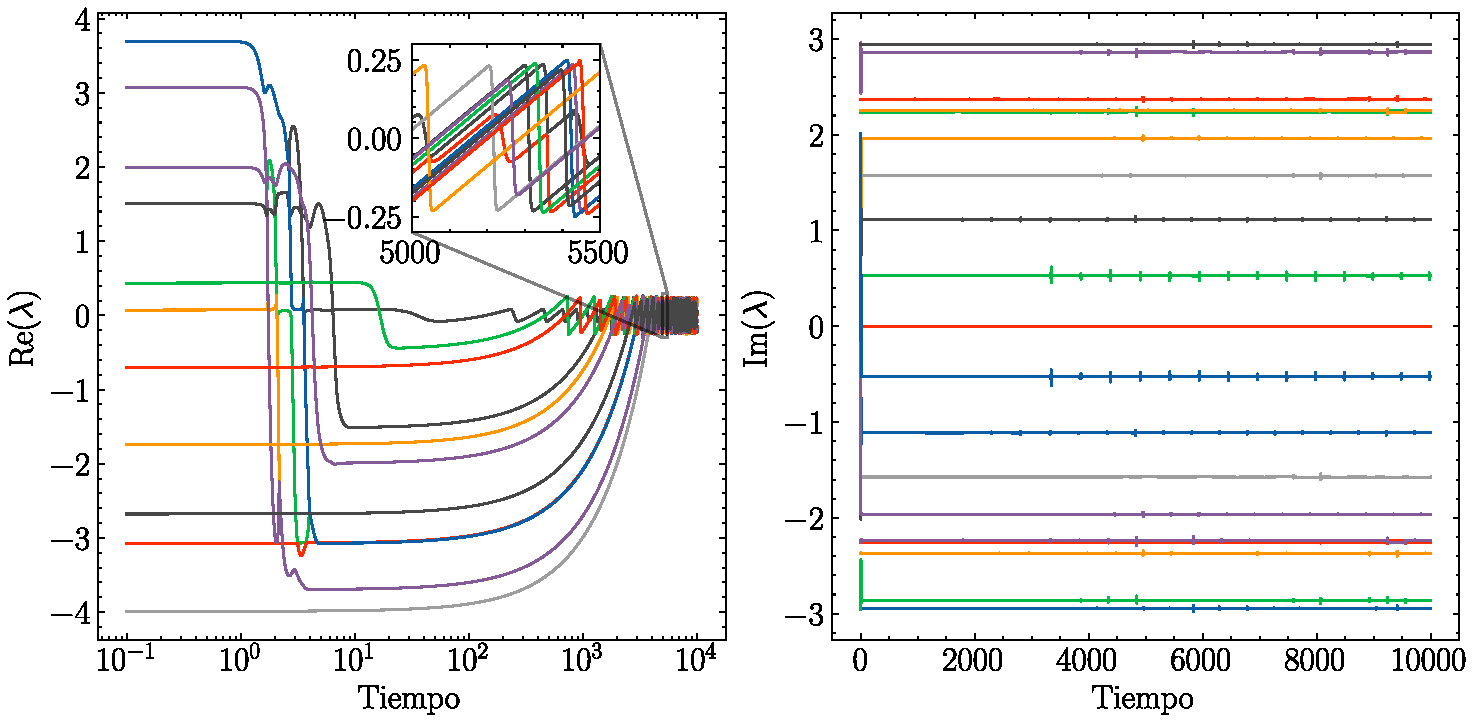
\includegraphics[width=\textwidth]{Figures/Evolucion coloreada.pdf}

    Como el término antihebbiano es simétrico, la parte imaginaria de los autovalores apenas es afectada, mientras que la parte real de los autovalores se coloca en torno a 0, en la región dinámicamente crítica.
\end{frame}

\begin{frame}{Ausencia de Criticidad Autoorganizada}
    \begin{columns}
        \begin{column}{0.5\textwidth}
            A pesar de la similitud en los nombres, un sistema que se autoorganiza a un régimen de {\color{blue}criticidad dinámica} no implica {\color{blue}criticidad autoorganizada}. La red neuronal carece de las propiedades necesarias

            \vspace{0.15in}

            \begin{itemize}
                \item Existencia de una escala característica
                \item Ausencia de \emph{scaling}
                \item Ausencia de leyes de potencias en el espectro de la matriz de covarianza.
            \end{itemize}
        \end{column}
        \begin{column}{0.45\textwidth}
        \centering
        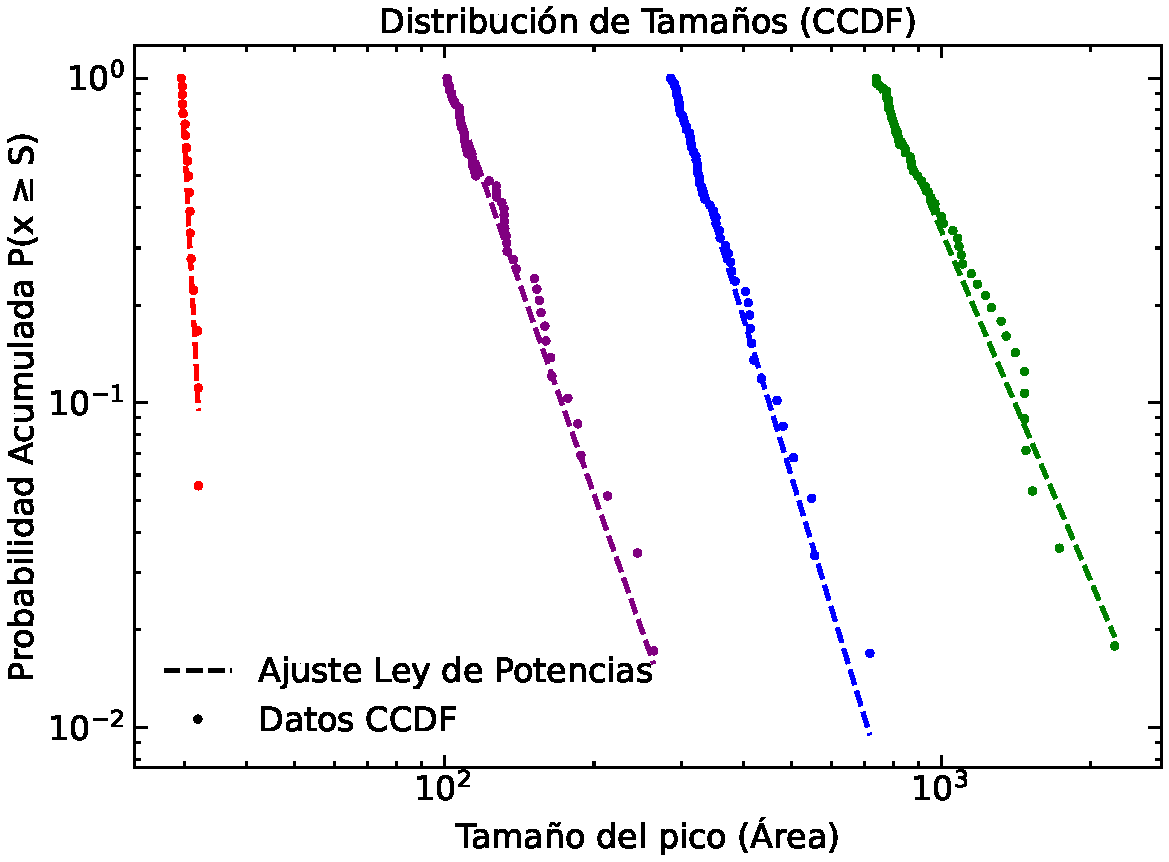
\includegraphics[width=\textwidth]{Figures/powerlaw.pdf}
        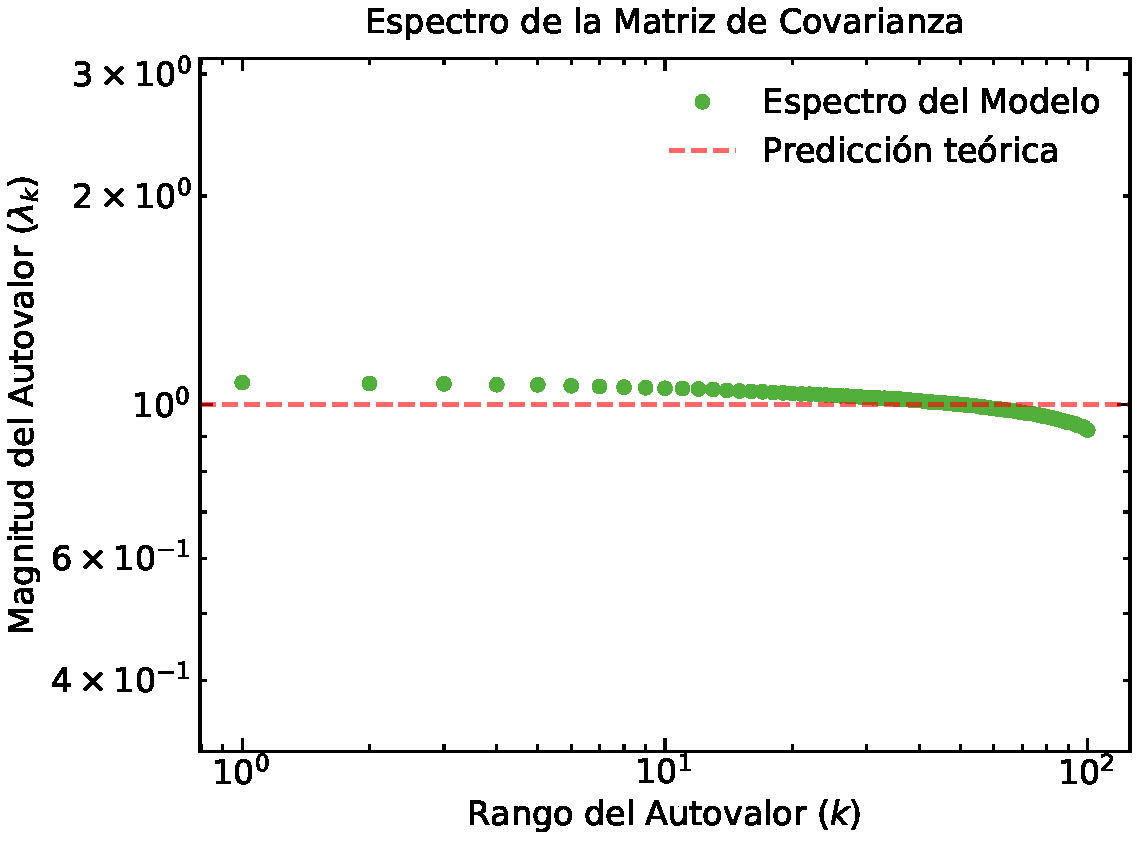
\includegraphics[width=\textwidth]{Figures/Espectro covarianza.pdf}
        \end{column}
    \end{columns}
\end{frame}

\begin{frame}{Aprendizaje Antisimétrico}
        \begin{columns}
        \begin{column}{0.5\textwidth}
            Como la homeostasis antihebbiana es {\color{blue}simétrica} es posible introducir aprendizaje de patrones en la parte {\color{blue}antisimétrica} de la matriz.

            Cada {\color{blue}memoria introducida} se compone de un {\color{blue}par de autovalores} complejo conjugados que se separa del resto en el eje imaginario, introducidos mediante el {\color{VerdeEstimulo}término de aprendizaje} en \(W\)

            \begin{eqbox}
                \begin{equation}
                    \dot{W} = \alpha (\mathbb{1} - \mathbf{xx}^T + {\color{VerdeEstimulo}\mathbf{uv}^T - \mathbf{vu}^T})
                \end{equation}                
            \end{eqbox}


        \end{column}
        \begin{column}{0.45\textwidth}
        \centering
        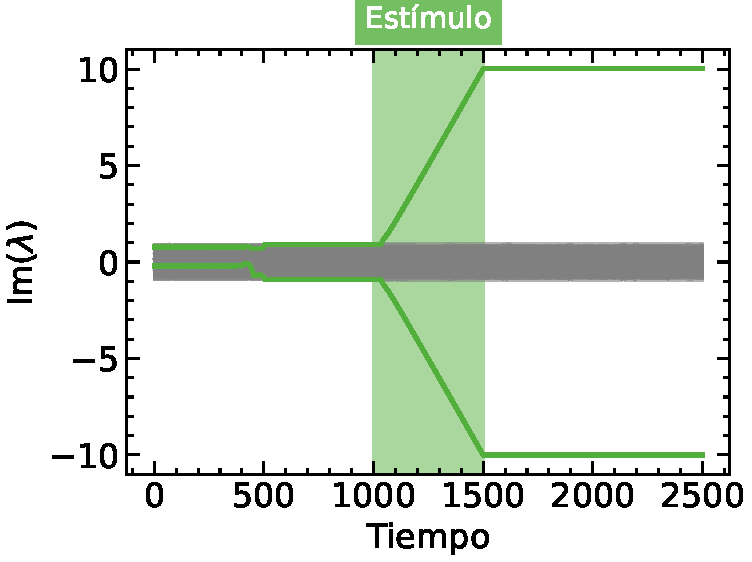
\includegraphics[width=\textwidth]{Figures/estimulo antisimetrico autovalores.pdf}
        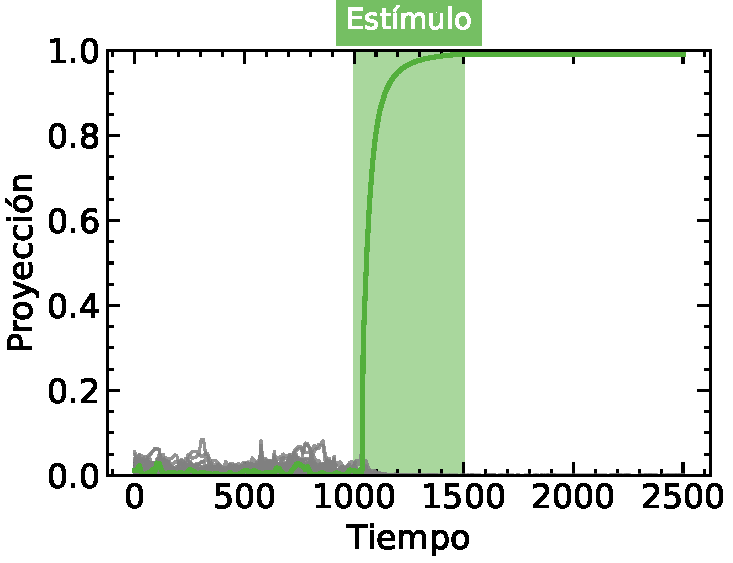
\includegraphics[width=\textwidth]{Figures/Estimulo antisimetrico proyeccion.pdf}
        \end{column}
    \end{columns}
\end{frame}

\begin{frame}{Aprendizaje Antisimétrico}
        \begin{columns}
        \begin{column}{0.5\textwidth}
            Como la homeostasis antihebbiana es {\color{blue}simétrica} es posible introducir aprendizaje de patrones en la parte {\color{blue}antisimétrica} de la matriz.

            Cada {\color{blue}memoria introducida} se compone de un {\color{blue}par de autovalores} complejo conjugados que se separa del resto en el eje imaginario, introducidos mediante el {\color{VerdeEstimulo}término de aprendizaje} en \(W\)

            \begin{eqbox}
                \begin{align*}
                    \dot{W} &= \alpha (\mathbb{1} - \mathbf{xx^T} + \mathbf{xy}^T - \mathbf{yx}^T)\\
                    \dot{\mathbf{y}} &= \frac{1}{\tau}(\mathbf{x} - \mathbf{y})
                \end{align*}                
            \end{eqbox}


        \end{column}
        \begin{column}{0.45\textwidth}
        \centering
        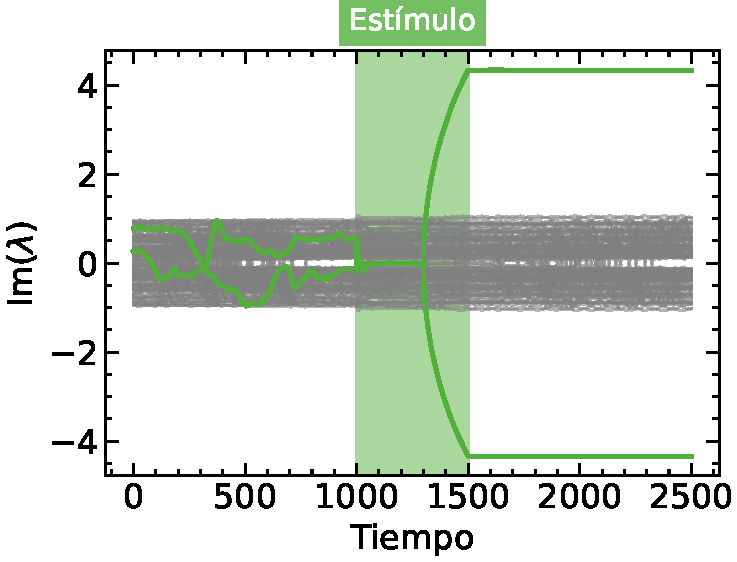
\includegraphics[width=\textwidth]{Figures/STDP correcto_cropped.pdf}
        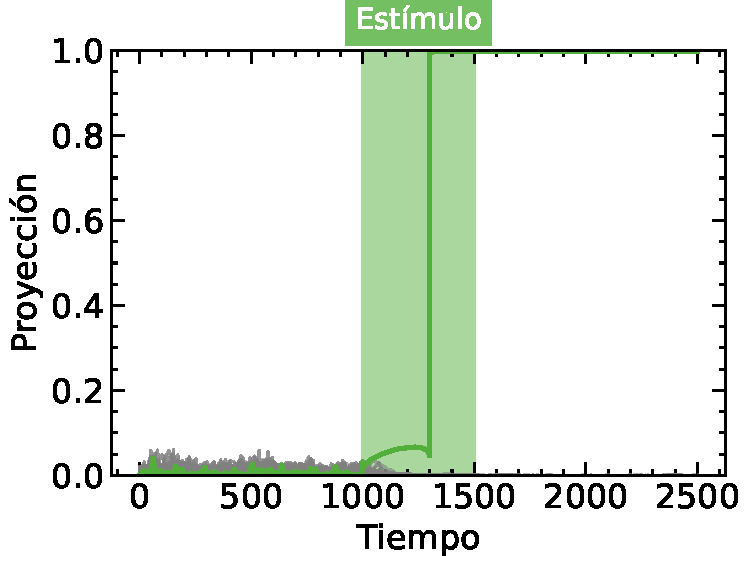
\includegraphics[width=\textwidth]{Figures/STDP correcto proyeccion.pdf}
        \end{column}
    \end{columns}
\end{frame}

\section{Conclusions}
\begin{frame}{Conclusions}
    
\end{frame}

\begin{frame}{Referencias}
    \printbibliography
\end{frame}

\end{document}